\documentclass[11pt,a4paper]{article}

\usepackage[colorlinks=true,pdftex]{hyperref}
\usepackage{latexsym}
\usepackage{amssymb}
\usepackage{amsmath}
\usepackage{amsfonts}
\usepackage{graphicx}
\usepackage{epsfig}
\usepackage{epstopdf}
\usepackage{esint}
\usepackage{hyperref}
\usepackage{amsthm}
\usepackage{mathtools}
\usepackage{color}
\usepackage[english]{babel}
\usepackage[utf8]{inputenc}
\usepackage{pdfpages}

\newcommand{\id}{\operatorname{id}}
\newcommand{\R}{\mathbb R}
\newcommand{\Z}{\mathbb Z}

\addtolength{\topmargin}{-3.5cm} \addtolength{\oddsidemargin}{-2cm}
\addtolength{\textheight}{+5cm} \addtolength{\textwidth}{+4cm}

\begin{document}
\hrule\hrule
\vspace{1mm}

\noindent {\bf Curso Avanzado de Geometría, 2024/25.
\hfill{Problem Set 2: The fundamental group}}

\vspace{1mm}

 \noindent {\bf Name}: Gonzalo Ortega Carpintero
\vspace{2mm}

\hrule\hrule

\subsection*{Exercise 1}
\begin{proof}
Let $X$ and $Y$ path-connected spaces. If $[\gamma] \in \pi_1(X \times Y, (x, y)) $, then $ \gamma \colon I \to X \times Y $ is a loop in the direct product pace where $ \gamma(0) = \gamma(1) = (x,y) $. We can write $ \gamma $ as
$
  \gamma(t) = (\gamma_X(t), \gamma_Y(t))
$
where $ \gamma_X \colon I \to X $ and $ \gamma_Y \colon I \to Y $ are loops in $ X $ and $ Y $ respectively with $ \gamma_X(0) = \gamma_X(1) = x $ and $ \gamma_Y(0) = \gamma_Y(1) = y $. Hence we can define the morphism
\begin{align*}
  f \colon \pi_1(X \times Y, (x, y)) &\to \pi_1(X, x) \times \pi_1(Y,y) \\
  [\gamma] &\mapsto ([\gamma_X], [\gamma_Y]).
\end{align*}
\begin{itemize}
  \item Let $*$ denote the path concatenation operator and let $ [\gamma_1], [\gamma_2] \in \pi_1(X \times Y, (x, y)) $, then
  \begin{align*}
    f([\gamma_1]\cdot[\gamma_2]) &= f([\gamma_1 * \gamma_2]) = ([(\gamma_1 * \gamma_2)_X], [(\gamma_1 * \gamma_2)_Y]) \\
    &= ([\gamma_{1X}], [\gamma_{1Y}]) \cdot ([\gamma_{2X}], [\gamma_{2Y}]) = f([\gamma_1]) \cdot f([\gamma_2])
  \end{align*}
  and $f$ is in fact an homomorphism.

  \item If $ ([\gamma_X], [\gamma_Y]) $ is the identity in $\pi_1(X, x) \times \pi_1(Y,y)$ then $ [\gamma_X] $ is the class of the constant path $ [\gamma_X] = [x_0]$. The same for $ [\gamma_Y] = [y_0]$. Therefore, if $ f([\gamma]) = ([x_0], [y_0]) $ then $ [\gamma] = [(x_0, y_0)] $ is also the identity in $ \pi_1(X \times Y, (x, y)) $. Hence, $ f $ is injective.
  
  \item For any pair of path classes $ [\alpha] \in \pi_1(X, x) $ and $ [\beta] \in \pi_1(Y,y) $ we can take the path $ \gamma(t) =(\alpha(t), \beta(t)) $ for which $ f([\gamma]) = ([\alpha], [\beta]) $. Hence, $ f $ is also surjective.
\end{itemize}
This makes $ f $ a isomorphism and $ \pi_1(X \times Y, (x, y)) \cong \pi_1(X, x) \times \pi_1(Y,y) $
\end{proof}

\subsection*{Exercise 7}
\renewcommand{\theenumi}{\alph{enumi}} 
\begin{enumerate}
  \item We have that $  \coloneq \mathbb R^3 \setminus \{\text{x-axis and y-axis}\} = \mathbb R^3 \setminus \{(x, 0, 0), (0, y, 0) : \forall x, y \in \mathbb R\} $. Defining the retraction $ r_1 $ such as 
  \begin{align*}
    r_1 \colon X &\to S^2 \setminus \{\pm (1, 0, 0), \pm (0, 1, 0) \} \\
    (x, y, z) &\mapsto \frac{(x, y, z)}{\sqrt{x^2 + y^2 + z^2}},
  \end{align*}
  we show that the space minus two axis is homotopic to the sphere without four points. Making a translation of one of the missing points of the sphere, we have that
  $$
    S^2 \setminus \{\pm (1, 0, 0), \pm (0, 1, 0) \} \cong S^2 \setminus \{(1, 0, 0), \pm (0, 1, 0), (0, 0, 1) \}
  $$
  and defining the retraction $r_2$ as the stereographic projection
  \begin{align*}
    r_2 \colon S^2 \setminus \{(1, 0, 0), \pm (0, 1, 0), (0, 0, 1) \} &\to \mathbb R^2 \setminus \{\pm (1, 0), (1, 0) \} \\
    (x, y, z) &\mapsto \left(\frac{y}{1-x}, \frac{z}{1-x}\right),
  \end{align*}
  we have that
  $
    X \simeq \mathbb R^2 \setminus \{\pm (1, 0), (1, 0) \} \simeq S^1 \vee S^1 \vee S^1 
  $
  and therefore
  $$
    \pi_1 (X) = \pi_1(S^1 \vee S^1 \vee S^1) = \mathbb Z * \mathbb Z * \mathbb Z.
  $$
  
  \item Without lose of generality, we can take $ X \coloneq \R^3 \setminus \{(x, 0, 0), (0, 1, 0) : x \in \R \} $. The open sets 
  \begin{align*}
    U &\coloneq \{(x, y, z) \in \R^3 : x < 2/3, y \neq 0 \text{ or } z \neq 0\} \\
    V &\coloneq \{(x, y, z) \in \R^3 : x > 1/3, (x, y, z) \neq (0, 1, 0) \}
  \end{align*} 
  are path-connected and $ U \cup V = X $. On one hand, we have that $ V $ and $ U \cap V $ are contractible, therefore $ \pi_1(V) = \pi_1(U \cap V) = \{ \cdot \} $. On the other hand, $ V \simeq S^1 $, and $ \pi_1(V) = \pi_1(S^1) = \Z$. Applying Seifert-Van Kampen theorem we have that
  $$
    \pi_1(X) = \pi_1(V) = \Z.
  $$

  \item The space $\R^3 $ without any two disjoint lines is homeomorphic to $\R^3 $ without two disjoint {\it parallel} lines. Without lose of generality, let $ X \coloneq \R^3 \setminus \{(x, 0, 0), (x, 1, 0) : x \in \R\} $. Using the retract
  \begin{align*}
    r \colon X &\to \R^2 \setminus \{(0, 0), (1, 0)\} \\
    (x, y, z) &\mapsto (y, z)
  \end{align*}
  we have that $ X \simeq \R^2 \setminus \{(0, 0), (1, 0)\} \simeq S^1 \vee S^1 $ and
  $$
    \pi_1(X) = \pi_1(S^1 \vee S^1) = \mathbb Z * \mathbb Z.
  $$
  
  \item Let $ X \coloneq T^2 - \{p, q\} $ be the torus minus two points. In Figure \ref{fig:7d} we make use of the diagrams seen in class to compute the fundamental group of the space. In step (1) we picture the diagram of the torus with two points removed. In (2) we contract one of the removed points to the boundary of the diagram while cutting one edge to the other point. Thus, in (3) we can see the obtained result. By deforming the diagram as in (4) and gluing the repeated edges $a$ and $b$ together we obtain the wedge of (5). That is, $ X \simeq S^1 \vee S^1 \vee S^1$ and 
  $$
  \pi_1(X) = \pi_1(S^1 \vee S^1 \vee S^1) = \mathbb Z * \mathbb Z * \mathbb Z.
  $$
\end{enumerate}
\begin{figure}[h]
  \centering
  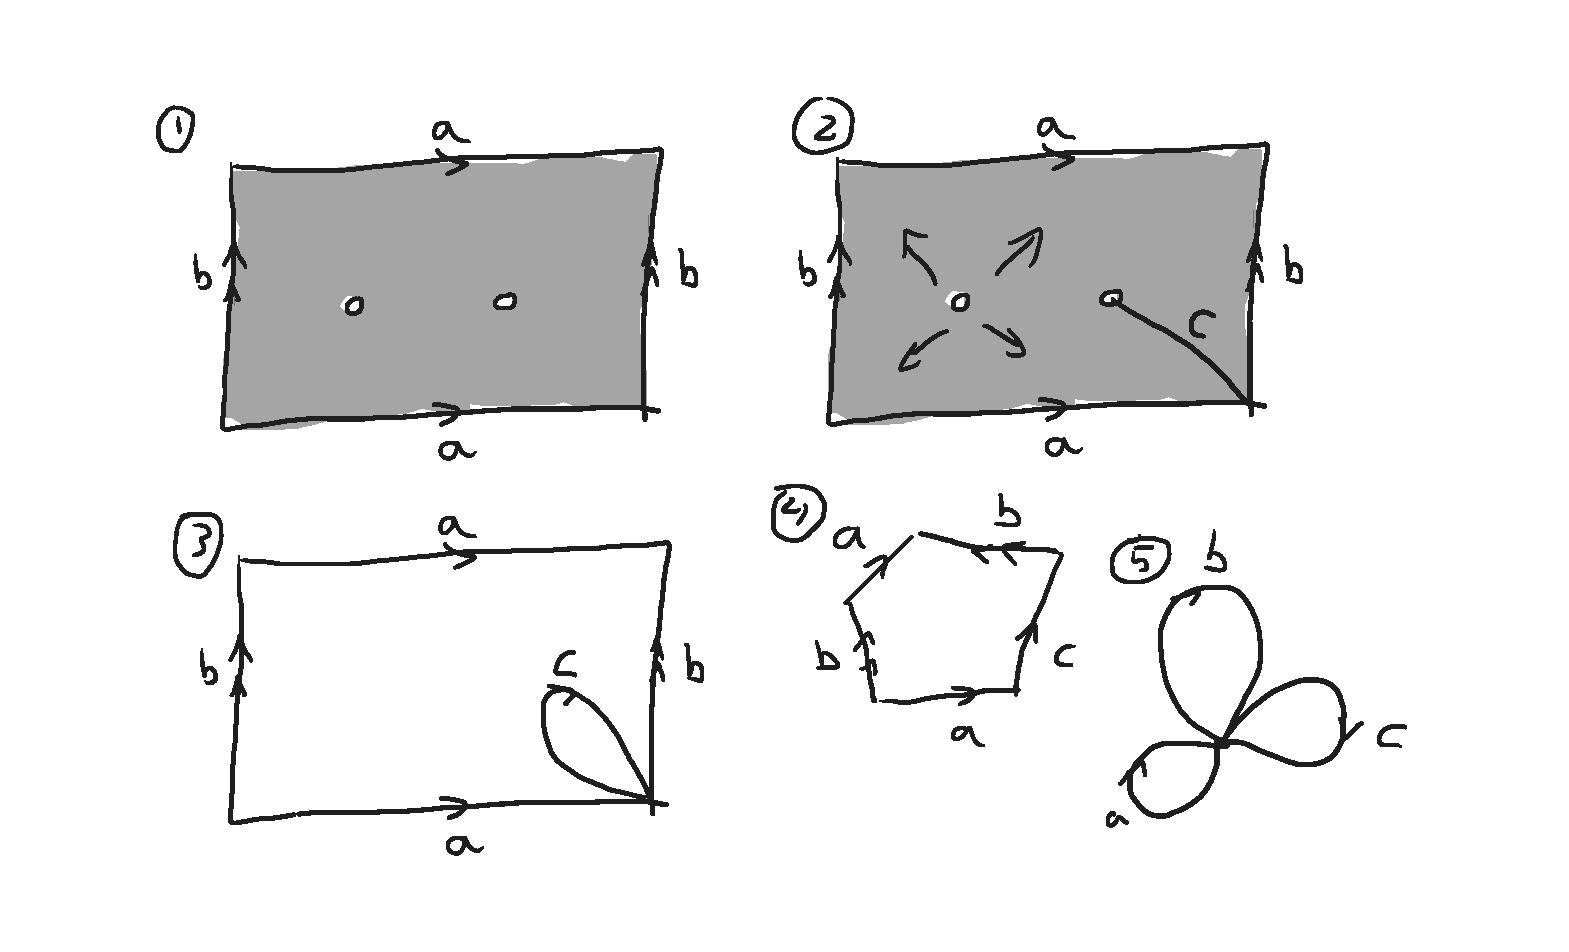
\includegraphics[width=15cm]{7d.pdf}
  \caption{Diagrams of the steps followed to compute the fundamental group of the torus $T^2$ minus two points.}
  \label{fig:7d}
\end{figure}

\section*{Exercise 8}
In Figure \ref{fig:63} we have chosen an orientation and numbered the under-crossings of the knot $ 6_3 $. Following the algorithm seen in class we compute the following Wirtinger relations. We denote (RH) the right hand crossings and (LH) the left hand ones. Note that we only need to compute the first 5, as the sixth can be computed as combinations of the previous ones.
\renewcommand{\theenumi}{\arabic{enumi}} 
\begin{enumerate}
  \item (RH) $ i_*(x_1) = a e b^{-1} e^{-1} $
  \item (LH) $ i_*(x_2) = b d^{-1} c^{-1} d $
  \item (LH) $ i_*(x_3) = c f^{-1} d^{-1} f $
  \item (RH) $ i_*(x_4) = d a e^{-1} a^{-1} $
  \item (LH) $ i_*(x_5) = e c^{-1} b^{-1} c $
\end{enumerate}
Hence, the Wirtinger presentation of $ \pi_1 (\R^3 \setminus 6_3) $ is
$$
  \langle a, b, c, d, e, f \mid a e b^{-1} e^{-1}, b d^{-1} c^{-1} d, c f^{-1} d^{-1} f, d a e^{-1} a^{-1}, e c^{-1} b^{-1} c\rangle.
$$
\begin{figure}[h]
  \centering
  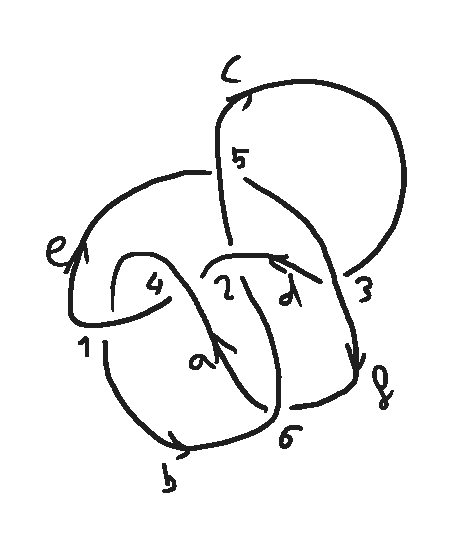
\includegraphics[width=5cm]{63.pdf}
  \caption{Knot $6_3$ with the chosen orientation and under-crossings numbered.}
  \label{fig:63}
\end{figure}

\section*{Exercise 10}
The Wirtinger presentation of the fundamental group of any knot complement in $ S^3$ is a presentation of the from
$$
  a
$$

\begin{thebibliography}{9}

  \bibitem{gath}
  Allen Hatcher,
  \textit{Algebraic Topology},
  Allen Hatcher 2001.

  \bibitem{nico}
  \textit{In Exercise 7.d., the cut made to obtain vertex $c$ was inspired by the one explained to me by Nicolas.}
  
\end{thebibliography}

\end{document}
